%%% пример отчета взян с сайта http://k806.ystok.ru/

\documentclass[15pt]{extarticle}

\usepackage{fullpage}
\usepackage{multicol,multirow}
\usepackage{tabularx}
\usepackage{ulem}
\usepackage[utf8]{inputenc}
\usepackage[russian]{babel}
\usepackage{amsmath}
\usepackage{amssymb}
\usepackage{graphicx}

% margin from paper borders
\usepackage[margin={0.8in, 0.3in}]{geometry}
% displaystyle в каждом мас моде
\everymath{\displaystyle}

\usepackage{titlesec}

\titleformat{\section}
  {\normalfont\Large\bfseries}{\thesection.}{0.3em}{}

\titleformat{\subsection}
  {\normalfont\large\bfseries}{\thesubsection.}{0.3em}{}

\titlespacing{\section}{0pt}{*2}{*2}
\titlespacing{\subsection}{0pt}{*1}{*1}
\titlespacing{\subsubsection}{0pt}{*0}{*0}
\usepackage{listings}
\lstloadlanguages{Lisp}
\lstset{extendedchars=false,
    breaklines=true,
    breakatwhitespace=true,
    keepspaces = true,
    tabsize=2
}



\begin{document}

\section*{Отчет по лабораторной работе №\,3
по курсу \guillemotleft  Функциональное программирование\guillemotright}

\begin{flushright}
Студент группы 8О-307 МАИ \textit{Гамов Павел}, \textnumero 4 по списку \\
\makebox[7cm]{Контакты: {\tt pagamov@gmail.com} \hfill} \\
\makebox[7cm]{Работа выполнена: 27.05.2021 \hfill} \\
\ \\
Преподаватель: Иванов Дмитрий Анатольевич, доц. каф. 806 \\
\makebox[7cm]{Отчет сдан: \hfill} \\
\makebox[7cm]{Итоговая оценка: \hfill} \\
\makebox[7cm]{Подпись преподавателя: \hfill} \\

\end{flushright}

\section{Тема работы}
Последовательности, массивы и управляющие конструкции Коммон Лисп

\section{Цель работы}
Научиться создавать векторы и массивы для представления матриц, освоить общие функции работы с последовательностями, инструкции цикла и нелокального выхода.

\section{Задание (вариант № 3.26/2)}
Запрограммировать на языке Коммон Лисп функцию, принимающую в качестве единственного аргумента двумерный массив, представляющий действительную матрицу A.
Функция должна возвращать новую матрицу B того же размера, каждый элемент которой bij равен наибольшему из элементов матрицы A, расположенных в области, определяемой индексами i и j и заштрихованной на рисунке.

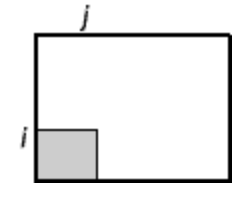
\includegraphics[scale=0.5]{pic}

\section{Оборудование студента}
macOS Catalina 10.15.7 Intel Core i5 2.3 GHz 8 ГБ RAM

\section{Программное обеспечение}
macOS, среда {\tt vim + sbcl}

\section{Идея, метод, алгоритм}
Используя методы динамического программирования делаем двойной цикл по матрице, начиная от левого нижнего края, проверяя два условия, является ли элемет ниже или левее больше чем текущий, если так, делаем замену, продолжаем пока не окажемся в правом верхнем углу.

\section{Сценарий выполнения работы}
Написал алгоритм на листочке, чтобы убедиться в корректности алгоритма. Написал функцию копирования и обработки массива в соответствии с требованием задачи.

\section{Распечатка программы и её результаты}

\subsection{Исходный код}

\begin{lstlisting}
(defun copy-array (arr)
  (let* ((dimensions (array-dimensions arr)) (new-arr (make-array dimensions)))
    (dotimes (i (array-total-size arr))
      (setf (row-major-aref new-arr i)
            (row-major-aref arr i)))
    new-arr))

(defun fun (mat)
  (let ((size (array-dimensions mat)))
    (let ((lines (first size)) (columns (second size)) (ans (copy-array mat)))
      (do ((i (- lines 1) (- i 1))) ((< i 0) ans)
        (do ((j 0 (+ j 1))) ((>= j columns) 'done_str)
          (if (and (> j 0) (> (aref ans i (- j 1)) (aref ans i j)))
            (setf (aref ans i j) (aref ans i (- j 1))))
          (if (and (< i (- lines 1)) (> (aref ans (+ i 1) j) (aref ans i j)))
            (setf (aref ans i j) (aref ans (+ i 1) j))
            ))))))

(print (fun (make-array '(3 3) :initial-contents '((0 1 2) (3 4 5) (6 7 8)) )))
(print (fun (make-array '(3 3) :initial-contents '((3 4 5) (2 3 4) (1 2 3)) )))
\end{lstlisting}

\subsection{Результаты работы}

\begin{lstlisting}
#2A((6 7 8) (6 7 8) (6 7 8)) 
#2A((3 4 5) (2 3 4) (1 2 3))
\end{lstlisting}

\section{Дневник отладки}

\begin{tabular}{|c|c|c|c|}
\hline
Дата     & Событие              & Действие по исправлению   & Примечание \\
27.05.21 & Написал алгоритм    & Разобрал все случаи &            \\
         & обработки матрицы &                           &            \\
\hline
\end{tabular}

\section{Замечания автора по существу работы}
Использование динамического программирования и циклов позволяют эффективно писать такие виды алгоритмов.

\section{Выводы}
Использование переменных и циклов не отличается от привычного Си языка, только в данном случае, компилятор очень сильно ругается на неиспользованные переменные, а также те, которые объявлять он считает опасным.

\end{document}
